% Licensed under the Creative Commons Attribution Share Alike 4.0 International.
% See the LICENSE file in the repository root for full license text.

\section{实验:构建包含多个源文件的程序}

包含多个源文件的 C++ 程序\emph{构建(build)}流程可以用图 \ref{fig:build-flow} 示意。该图将构建流程概括为以下三个步骤。

\begin{enumerate}
	\item \emph{预处理(preprocess)}。\emph{预处理器(preprocessor)}处理源文件中的 \lstinline[language={[17]C++}]{#include}、\lstinline[language={[17]C++}]{#define} 等预处理指令,对 \lstinline[language={[17]C++}]{#include} 指令、宏指令进行\textbf{文本替换}。
	\item \emph{编译(compile)}。\emph{编译器(compiler)}\textbf{独立地}处理各源文件,将每个源文件编译为中间文件。
	\item \emph{链接(link)}。\emph{链接器(linker)}处理\textbf{所有}需要的中间文件,最后生成可执行文件。
\end{enumerate}

\begin{figure}
	\centering
	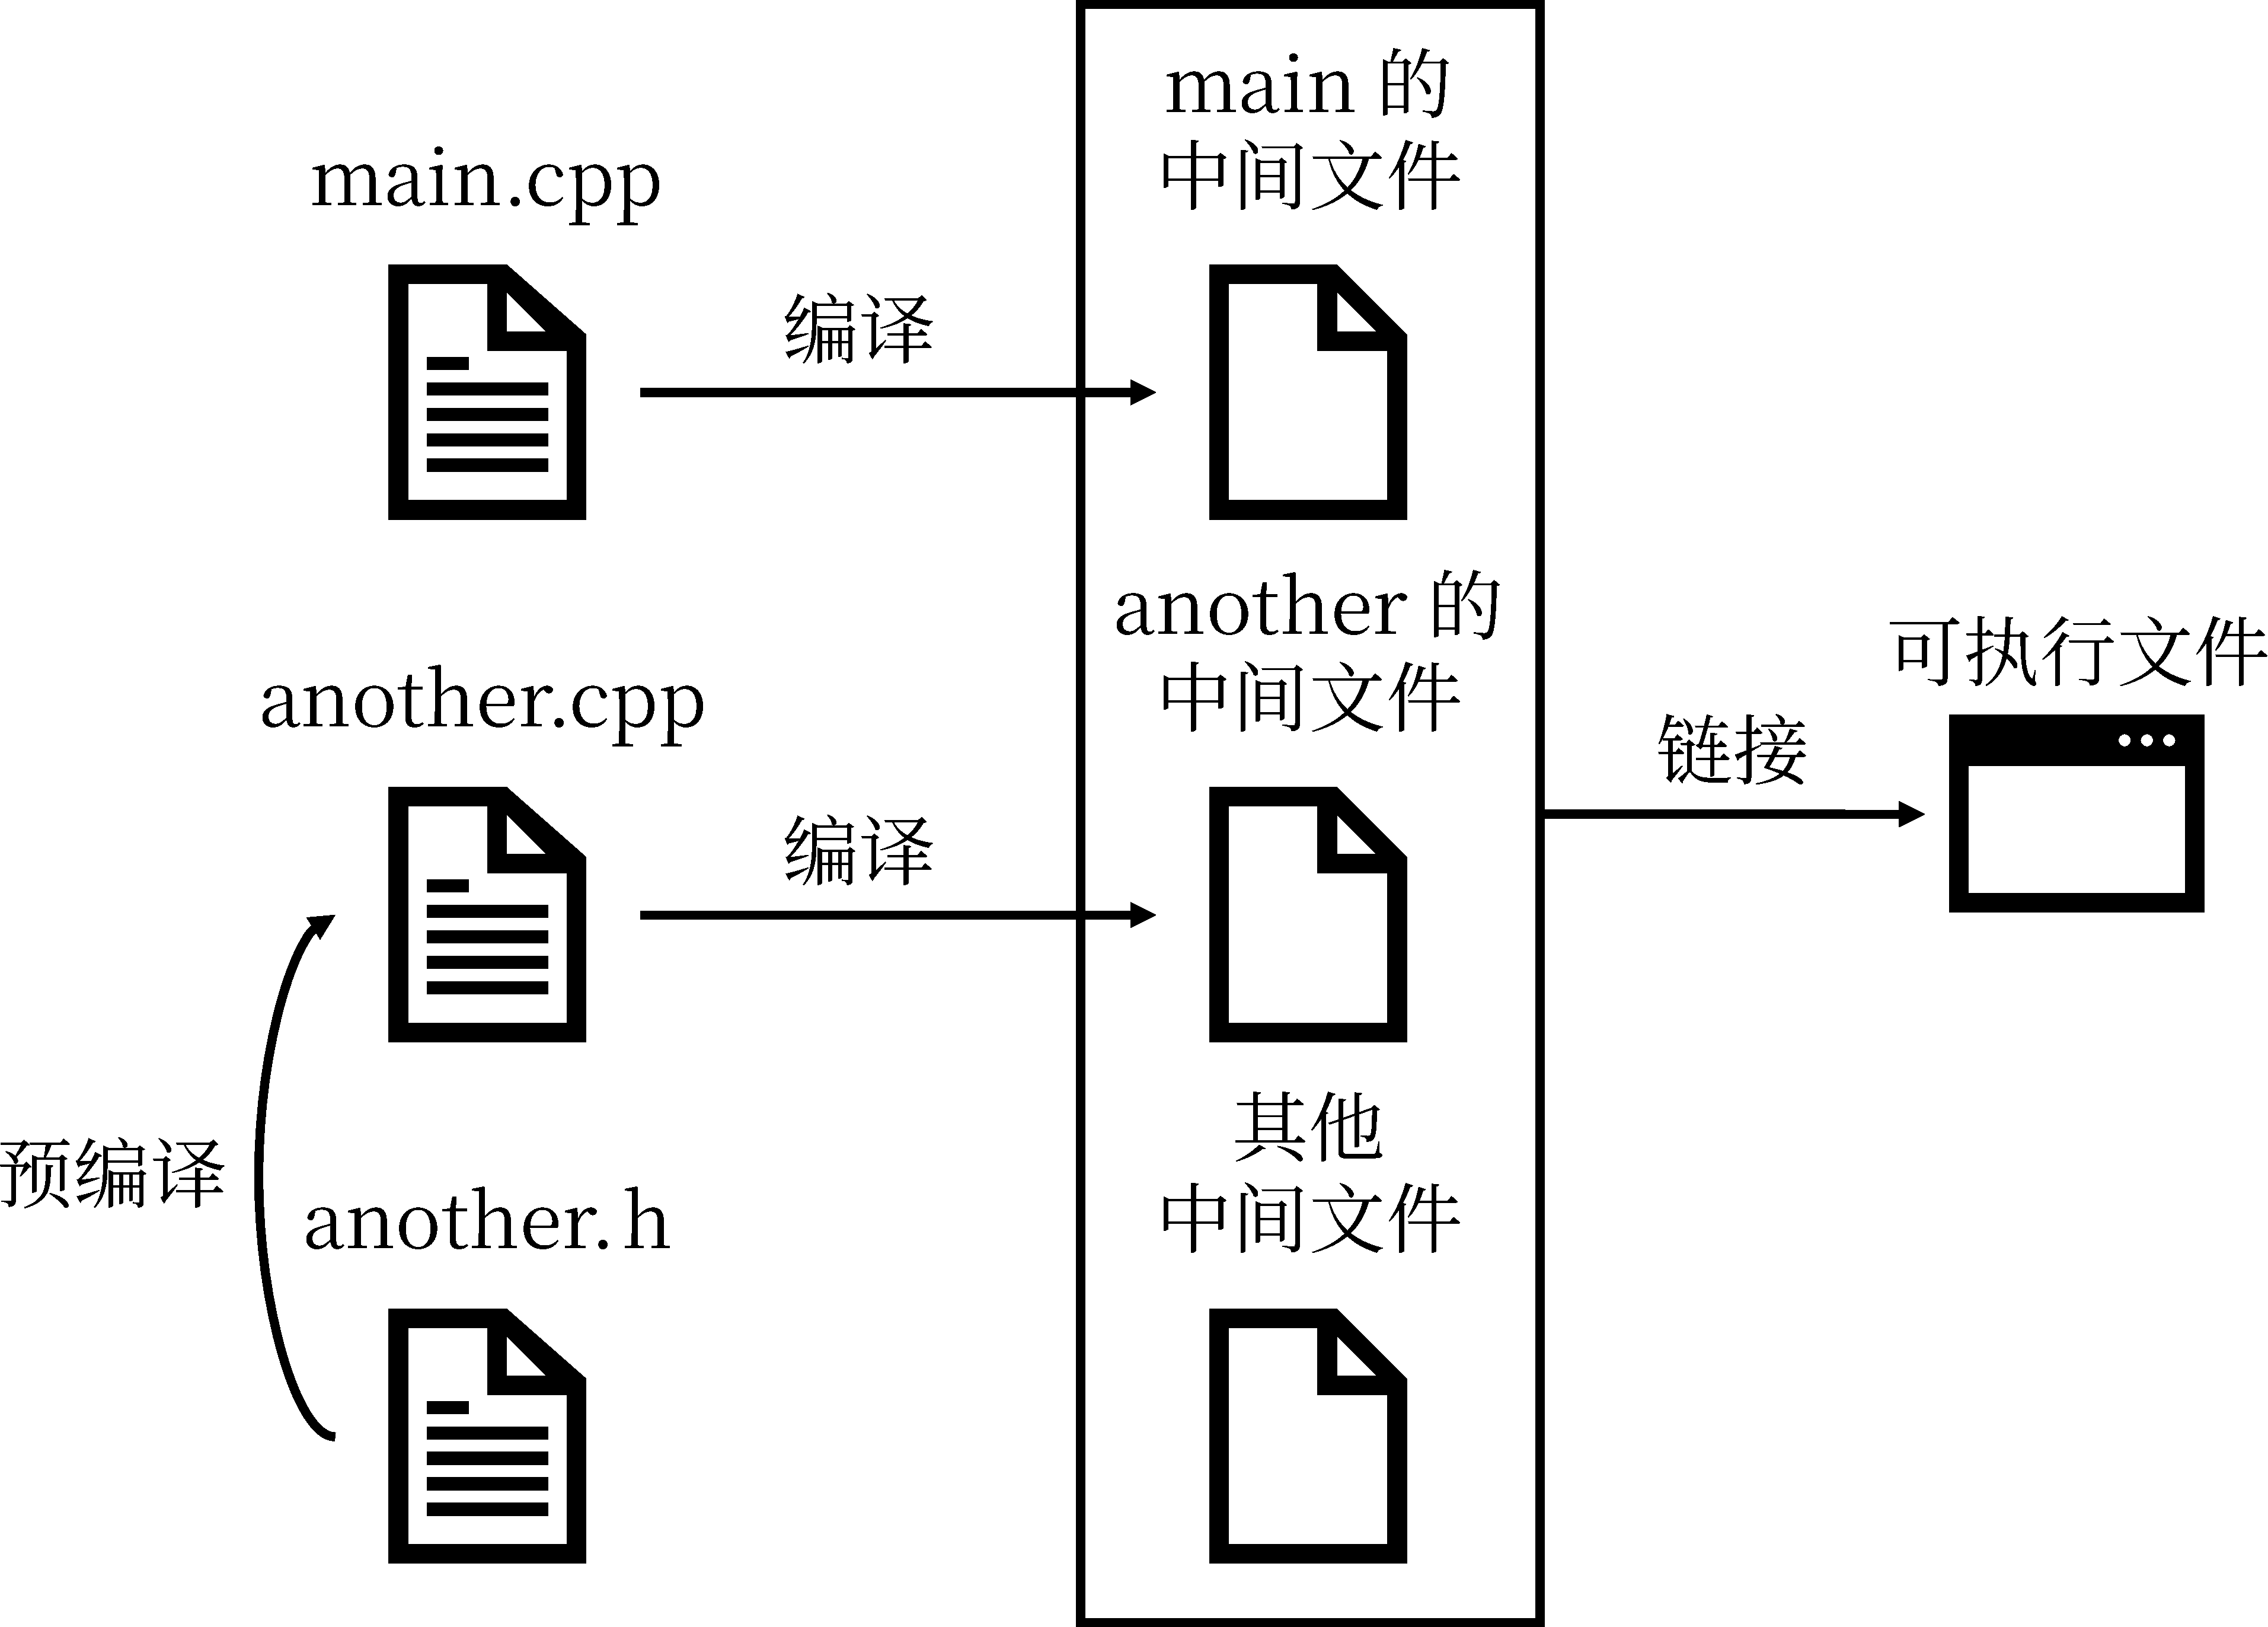
\includegraphics[scale=0.15]{assets/build-flow}
	\caption{多个 C++ 源文件的构建流程示意图。}
	\label{fig:build-flow}
\end{figure}

一般认为,C++ 程序的构建流程\footnote{没有讨论单个源文件经过编译得到单个中间文件时,习惯上用“编译”替代“构建”。}包括预处理、编译、汇编、链接四个步骤,此处我们将汇编这一步骤并入编译,以突出之后的实验要讨论的问题。

\subsection*{实验步骤}

\begin{enumerate}
	\item 新建项目。打开 Dev-C++,点击菜单栏中的“文件”、“新建”、“项目”,选择“Empty Project”,并为项目取一个好名称,如图 \ref{fig:multi-source-1} 所示。然后点击确定,通过“另存为”对话框选择项目保存的路径。

	\begin{figure}
		\centering
		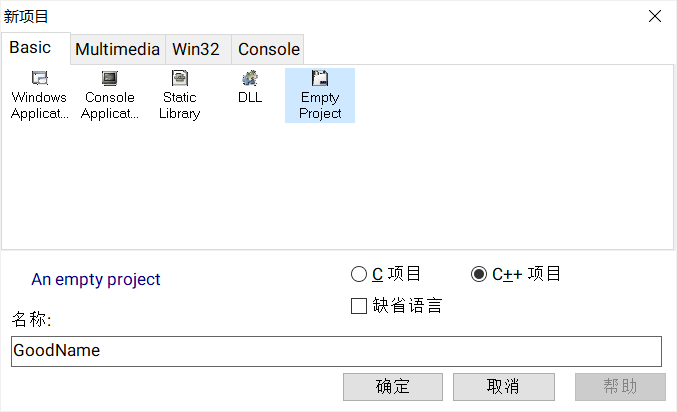
\includegraphics[width=0.75\linewidth]{assets/multi-source-1}
		\caption{新建项目对话框。}
		\label{fig:multi-source-1}
	\end{figure}

	\item 新建源文件。在“项目管理”窗口中,右键点击项目,点击弹出菜单中的 “New File”。立即保存新建的文件到默认路径,并为它取一个好名称。重复该步骤,得到如图 \ref{fig:multi-source-2} 所示的结果。

	\begin{figure}
		\centering
		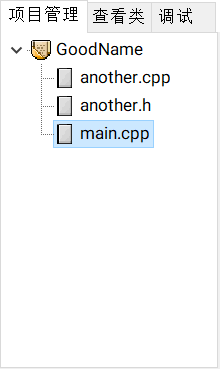
\includegraphics[width=0.2\linewidth]{assets/multi-source-2}
		\caption{新建源文件后的“项目管理”窗口。}
		\label{fig:multi-source-2}
	\end{figure}

	\item 编写代码。

	\begin{lstlisting}[language={[17]C++}]
// main.cpp
#include <iostream>

#include "another.h"

int main()
{
	long long ago { another("figure emerged") };
	std::cout << ago << std::endl;
}
	\end{lstlisting}

	\begin{lstlisting}[language={[17]C++}, moreemph={[2]another}]
// another.h
long long another(const char*);
	\end{lstlisting}

	\begin{lstlisting}[language={[17]C++}, moreemph={[2]another, strlen}]
// another.cpp
#include <cstring>

long long another(const char* str)
{
	return std::strlen(str);
}
	\end{lstlisting}

	\item 编译并运行代码。点击菜单栏中的“运行”、“编译运行”,可以看到“编译日志”窗口弹出,调用的命令记录如下。

	\begin{lstlisting}[language={}]
生成 makefile...
--------
- 文件名: C:\Users\lyche\Desktop\GoodName\Makefile.win

正在处理makefile...
--------
- makefile处理器: C:\Program Files (x86)\Embarcadero\Dev-Cpp\TDM-GCC-64\bin\mingw32-make.exe
- 命令: mingw32-make.exe -j16 -f "C:\Users\lyche\Desktop\GoodName\Makefile.win" all

g++.exe -c another.cpp -o another.o -I"C:/Program Files (x86)/Embarcadero/Dev-Cpp/TDM-GCC-64/include"

g++.exe -c main.cpp -o main.o -I"C:/Program Files (x86)/Embarcadero/Dev-Cpp/TDM-GCC-64/include"

g++.exe another.o main.o -o GoodName.exe -L"C:/Program Files (x86)/Embarcadero/Dev-Cpp/TDM-GCC-64/lib" -static-libgcc
	\end{lstlisting}
\end{enumerate}

\subsection*{讨论}

\begin{enumerate}
	\item
\end{enumerate}
